\documentclass{beamer}
\usetheme{Madrid}
\usecolortheme{beaver}

% Set graphics location
\graphicspath{ {Images/} }

%Information to be included in the title page:
\title{Structural Quality \& Software Evolution}
\author{Alison Major}
\institute{Lewis University}
\date{2022}

% \logo{
%   
\includegraphics[width=0.2\textwidth]{UniversityLogo}
% }

\begin{document}

\frame{\titlepage}

% 1 Introduction
% 1.1 Maintainability Index and Pylint Refactor Scores
% 1.2 Paper Structure
\begin{frame}
  \frametitle{Introduction}
  \textbf{Maintainability Index and Refactor Scores}
  \begin{itemize}
    \item Areas of concern: cost, timeline, quality
    \item Quality is hard to understand
    \item Pylint \& Radon are a static analysis tools
    \item Refactor violations point out code smells
  \end{itemize}
\end{frame}

% 2 Background and Literature Review

% 2.1 Keeping Users Engaged Long Term
% 2.1.1 Why does software evolution matter?
% 2.1.2 How do we ensure software evolution?
\begin{frame}
  \frametitle{Keeping Users Engaged Long Term}
  \textbf{Why does software evolution matter?}
  \begin{itemize}
    \item Users find bugs
    \item Users want new features
    \item New security threats
    \item New laws from governing bodies
  \end{itemize}
  
  \vspace{0.35cm}
  Need a thriving community of engaged users in order to keep apps and games successful.

  \vspace{0.35cm}
  In an open source system, need a thriving community of engaged developers in order to continue evolving.
\end{frame}

\begin{frame}
  \frametitle{Keeping Users Engaged Long Term}
  \textbf{How do we ensure software evolution?}

  \vspace{0.35cm}
  Keep the project maintainable.
  \begin{itemize}
    \item Bugs should be quick and easy to fix
    \item New features should be easy to add
  \end{itemize}

  \vspace{0.35cm}
  \textbf{Software Maintenance}
  \begin{itemize}
    \item Consistent standards (naming, small methods, etc)
    \item Large portion of project cost in a typical software system is in the maintenance phase
  \end{itemize}
\end{frame}

\begin{frame}
  \frametitle{The Impact of Structural Quality}
  \textbf{Measuring Maintainability}
  \begin{itemize}
    \item easy to maintain = easy to evolve
    \item Pylint \& Radon Maintainability Index (MI)
  \end{itemize}

  \vspace{0.35cm}
  \textbf{Maintainability Scores}
  \begin{itemize}
    \item Refactor Messages (Pylint) --- code smells
    \item Code smells point out problems in Architecture
    \item PEP 8 is a set of Python standards
  \end{itemize}
\end{frame}

\begin{frame}
  \frametitle{The Impact of Structural Quality}
  \textbf{Other Maintainability Characteristics}
  \begin{itemize}
    \item Low coupling, high cohesion
    \item Confidence that metrics around software structure provide value in keeping systems maintainable (and therefore can evolve) % \cite{zhou:2020}
    \item Readability
    \begin{itemize}
      \item Big commits reduce maintainability
      \item PEP 8 enforces readability
    \end{itemize}
  \end{itemize}
\end{frame}

\begin{frame}
  \frametitle{The Impact of Structural Quality}
  \textbf{Documentation and Maintainability}
  \begin{itemize}
    \item Documentation holds the results of significant design decisions
    \item Can influence the ability to evolve because\dots
    \begin{itemize}
      \item Enhances code understanding
      \item Comprehensibility impacts maintainability in a positive way  
    \end{itemize}
  \end{itemize}
\end{frame}

\begin{frame}
  \frametitle{Related Work}
  \textbf{Design Patterns and Software Quality}
  \begin{itemize}
    \item Design patterns provide flexibility
    \item Classes with frequent changes
    \begin{itemize}
      \item Easy to extend (okay)
      \item Correlates to other classes (high coupling... red flag!)
    \end{itemize}
    \item We look at refactor score (code smell) not error score (bugs)
  \end{itemize}
  
  \vspace{0.35cm}
  Keeping this in mind, we focus on \emph{changes for system extensions and adaptiation}, not bug fixes.
\end{frame}

\begin{frame}
  \frametitle{Related Work}
  \textbf{Software Architecture and Maintainability}
  \begin{itemize}
    \item Maintainability
    \item Extensibility
    \item Simplicity, understanding
    \item Re-usability
    \item Performance
  \end{itemize}

  \vspace{0.35cm}
  Keep these in mind for easier future development 
  \newline when adding or changing code.
\end{frame}

% 3 Methodology
% 3.1 Initial Repository Set
% 3.2 Filtered Respository Set
\begin{frame}
  \frametitle{Methodology}
  \textbf{Initial Repository Set}
  \begin{itemize}
    \item Popular
    \item Long development history
    \item Multiple release cycles
  \end{itemize}

  \vspace{0.35cm}
  \textbf{Filtered Respository Set}
  
  \emph{At least 80\% Python code and top 20th percentile in these categories:}
  \begin{itemize}
    \item Long history of commits (2,968+ commits)
    \item Large number of contributors (90+ contributors)
    \item Many releases (44+ releases)
    \item Substantial Age (66.4+ months)
  \end{itemize}

  \vspace{0.35cm}
  Results in 46 repositories for further research.
\end{frame}

% 4 Results
\begin{frame}
  \frametitle{Results}
  \begin{itemize}
    \item Radon MI for all repositories rank as grade ``A''
    \newline which is considered ``very high maintainability''
    \item Open source systems with engaged community 
    \newline of developers tend to have higher scores
  \end{itemize}

  \vspace{0.35cm}
  To normalize, calculated ratio of refactor message count to SLOC.
  
  \vspace{0.35cm}
  \begin{itemize}
    \item Worst Score: \textbf{Raven-Python} - now deprecated
    \item Best Score: \textbf{Cython} - still active development
  \end{itemize}
\end{frame}

\begin{frame}
  \frametitle{Results}
  \begin{center}
    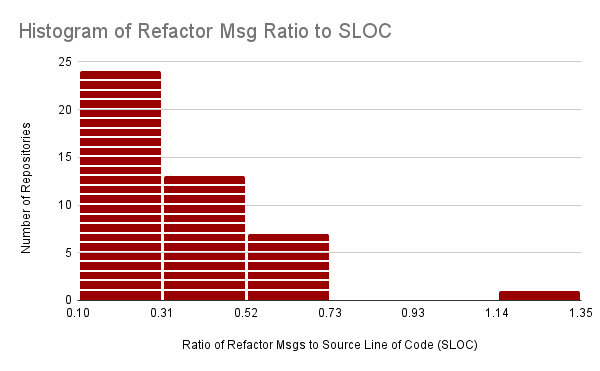
\includegraphics[width=0.8\columnwidth]{Histogram of Refactor Msg Ratio to SLOC.png}
  \end{center}
  \begin{center}
    {\small \emph{Diligent development communities can keep refactor warnings low,}}
    
    {\small \emph{regardless of system size (lines of code).}}
  \end{center}
\end{frame}

\begin{frame}
  \frametitle{Results}
  \begin{center}
    % 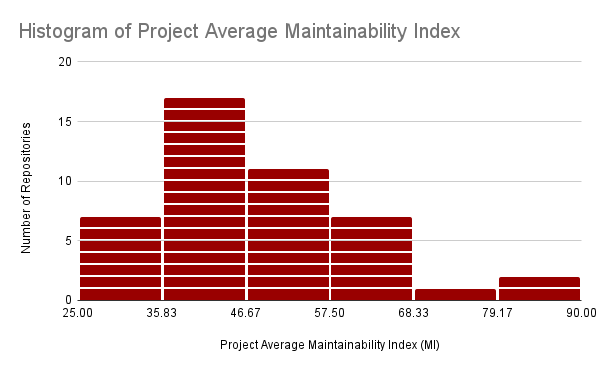
\includegraphics[width=0.8\columnwidth]{Histogram of Project Average Maintainability Index.png}
    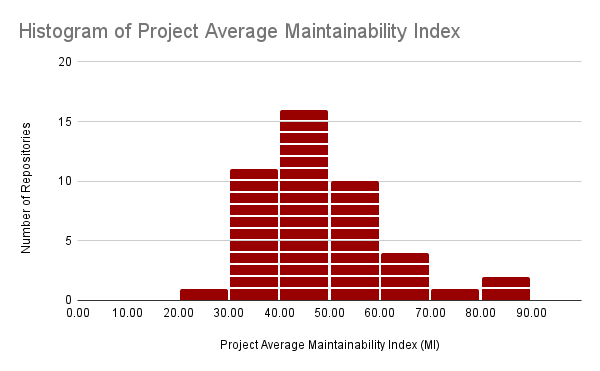
\includegraphics[width=0.8\columnwidth]{Histogram of Project Average Maintainability Index_BucketSize_10.png}
  \end{center}
  \begin{center}
    {\small \emph{Many repositories average in the mid-score to high-score.}} 
    
    {\small \emph{Radon considers 20 points and up to be very maintainable.}}
  \end{center}
\end{frame}

% 5 Conclusions and Recommendations
\begin{frame}
  \frametitle{Conclusions}
  \begin{itemize}
    \item Good projects will grow and evolve.
    
    \vspace{0.35cm}
    \item Structural quality impacts software evolution.
    
    \vspace{0.35cm}
    \item Poor structure leads to deprecation.
    \newline {\small \emph{(if the development community is engaged, deprecation of \newline the project may lead to a fresh, improved code base)}}
    
    \vspace{0.35cm}
    \item Open source and many contributor projects are vulnerable to degrading maintainability.
  \end{itemize}
\end{frame}

\begin{frame}
  \frametitle{Recommendations}
  \begin{itemize}
    \item Reliable metric can be useful.
    
    \vspace{0.35cm}
    \item Good architecture is important for evolution.
    
    \vspace{0.35cm}
    \item Pick a set of standards and auto-enforce to maintain good architecture even with a large, open source community.
  \end{itemize}
\end{frame}

\end{document}